\section{Generalized Critic Policy Optimization}
\label{sec:method}

%Test the method with different algorithms
%they need to be actor-critic algorithms
%will our method be implemented differently to include each algorithm's tricks? or will we only implement it on top of algorithms that do not require modifications?

%tableaux : lignes: algorithmes2baz, algorithmes + amélioration, algorithmes + améliorations d'autres articles. colonnes : tasks

%\begin{tabular}
%\end{tabular}
fsd 
\begin{figure}[!htb]
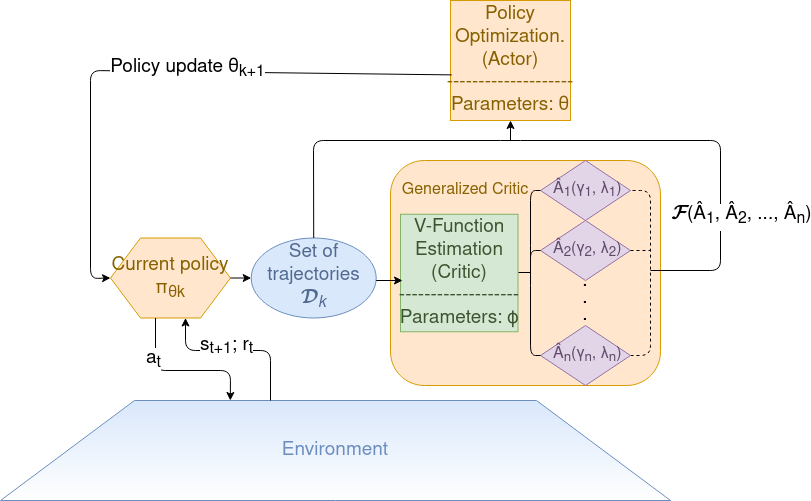
\includegraphics[width=8.5cm]{images/model}
\caption{Multi-advantage critic}
\label{fig:model}
\end{figure}
